The ability to perceive and reason about the world's actors, actions, objects, and relationships has been a longstanding goal for Computer Vision. 
Traditionally, we have benchmarked progress towards this goal using tasks like visual question answering~\cite{antol2015vqa}, in which a model's reasoning skills are evaluated by it's ability to answer questions about visual stimuli. 
A variety of benchmarks have been created to test a model's capabilities at answering questions about images~\cite{johnson2017clevr,hudson2019gqa,antol2015vqa,zellers2019recognition,goyal2017making,krishna2017visual,zhu2016visual7w,kim2020answering} and about videos~\cite{tapaswi2016movieqa,lei2018tvqa,jang2017tgif,kim2017deepstory,xu2017video,maharaj2017dataset,zeng2016leveraging,yu2019activitynet, yi2019clevrer, mun2017marioqa}. 
Ideally, models trained on these benchmarks should be capable of reasoning over both spatial relationships between objects~\cite{krishna2017visual,lu2016visual} and temporal ordering of actions~\cite{zacks2001events,ji2020action}. 
Unfortunately, since most question-answering benchmarks operate over images, they are limited to only testing spatial relationships (e.g.~"What is on top of the table?")~\cite{hudson2019gqa,krishna2017visual,antol2015vqa} or at most guessing common sense events occurring before and after the image~\cite{park2020visualcomet,zellers2019recognition}. 
The few existing video benchmarks have questions only use simple temporal logic (e.g."What does the bear on right do after sitting?")~\cite{jang2017tgif,xu2017video,maharaj2017dataset,zeng2016leveraging,yu2019activitynet}. 
However, to answer questions that require models to jointly compose spatial and temporal reasoning in more complex questions (e.g."What did they do to the last object they put down before opening the window?"), we need newer benchmarks and a new class of models.


\begin{figure}[t]
    \centering
    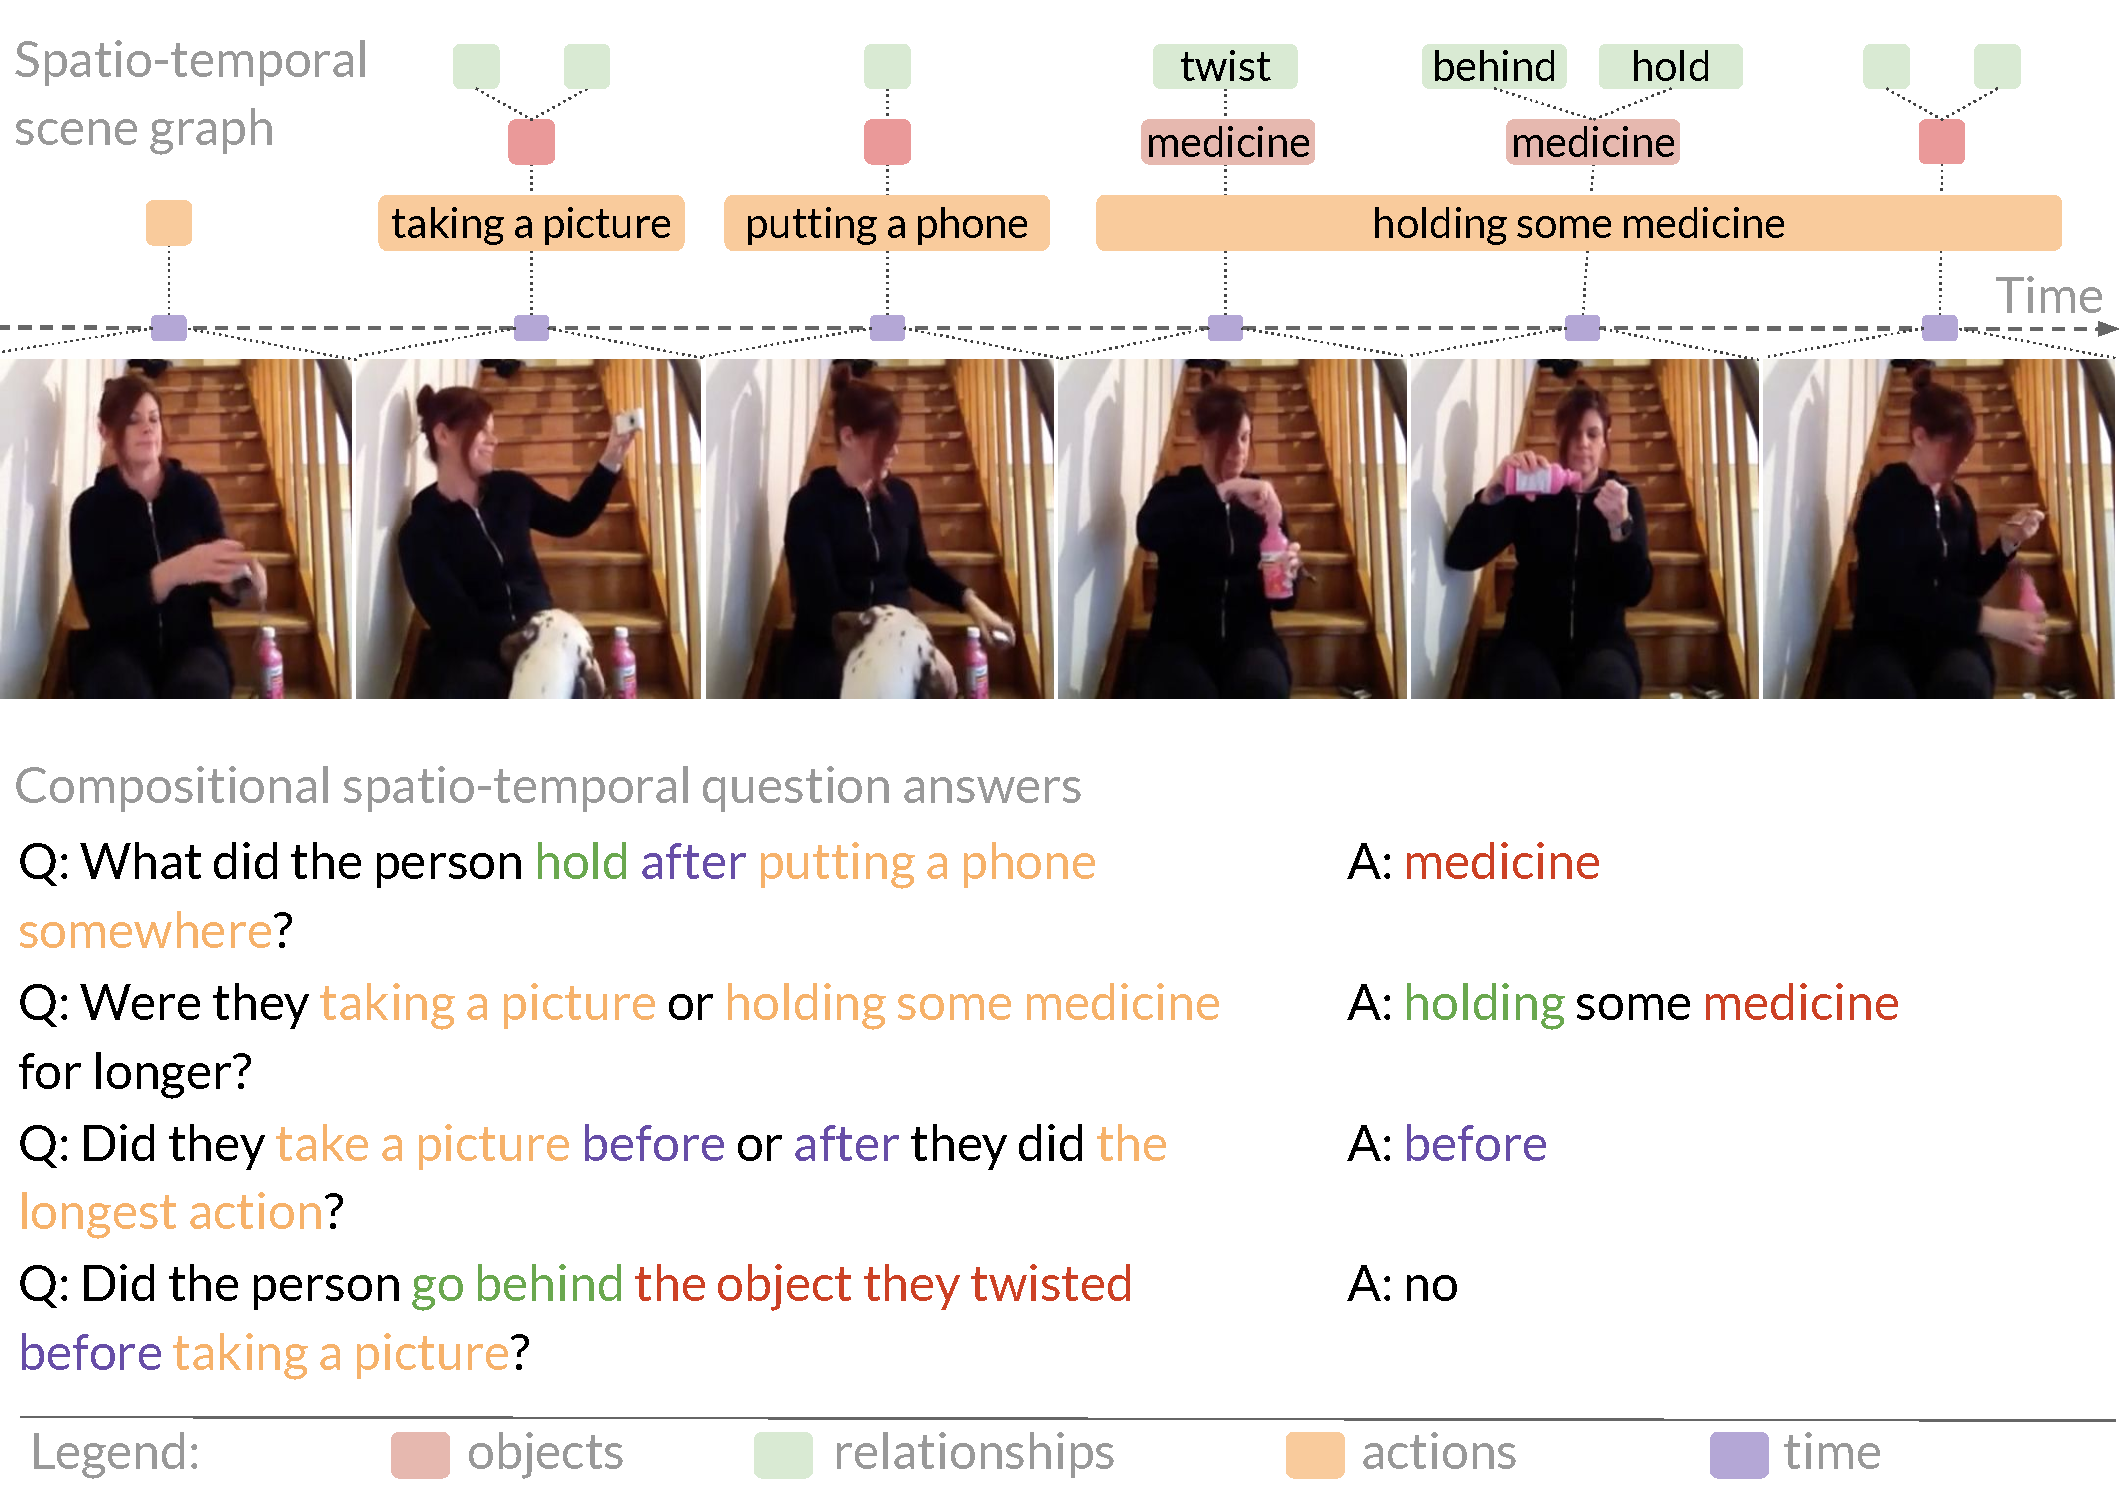
\includegraphics[width=\columnwidth]{figures/pull.pdf}
    \caption{We introduce AGQA: a new benchmark to test for compositional spatio-temporal reasoning. AGQA contains a balanced benchmark of 1.77M question answer pairs associated with 10K videos and an unbalanced set of 133M question answers in total. We argue that existing benchmarks do not test for compositional spatio-temporal reasoning and find that existing video question answering models do not demonstrate compositional capability.}
    \label{fig:pull}
\end{figure}

Meanwhile, Cognitive Science postulates that people actively encode events into structures characterized by systematic compositionality~\cite{michotte2017perception,barker1951one,zacks2001perceiving} --- the algebraic ability to comprehend a combinatorial number of novel combinations from known components. Once we learn to identify objects like \object{medicine}, understand relationships like \relationship{holding}, and recognize actions like \action{putting a phone somewhere}, we can compose these ideas together to explain when someone is \relationship{holding} \object{medicine} \temporal{before} \action{putting a phone somewhere}  (Figure~\ref{fig:pull}). This compositional ability is reflected in the language we use to communicate with one another~\cite{chomsky2002syntactic,montague1970universal}, allowing us the ability to showcase compositional reasoning and generate tests to check for this ability. We can ask questions like ``What did the person \relationship{hold} \temporal{after} \action{putting a phone somewhere}?'' and expect someone capable of compositional spatio-temporal reasoning to answer ``\object{medicine}''. While
that was a relatively simple composition, more complex questions can involve reasoning over novel combinations involving many different types of objects, spatial relationships, and temporal actions. While such compositional behavior seems fundamental to developing vision models that can reason over events in the world, we have only developed compositional benchmarks using static images~\cite{hudson2019gqa} or synthetic worlds~\cite{lake2018generalization,yi2019clevrer} which either are not spatio-temporal or do not reflect the diversity of real-world events.

Creating a benchmark for spatio-temporal questions is a challenging endeavor. It requires (1) identifying the core primitives that can be composed together, (2) be linguistically diverse enough to measure a variety of reasoning skills, (3) be minimally biased to prevent simple solutions, and (4) be capable of testing a variety of compositional metrics. 
Questions automatically generated from video captions often lack diversity in structure~\cite{yu2019activitynet,jang2017tgif}, while human annotations are too expensive to get a large enough sample devoid of biases in language or concepts~\cite{zeng2016leveraging,yu2019activitynet}. Additionally, generating a benchmark that allows us to test compositional behavior must contain a training\/test split where particular compositions only occur in the test set. Producing annotation workflows to adhere to such explicit splits requires specialized interfaces, tedious annotation verification, and is largely unexplored in the crowdsourcing literature.

\begin{figure}[t]
    \centering
    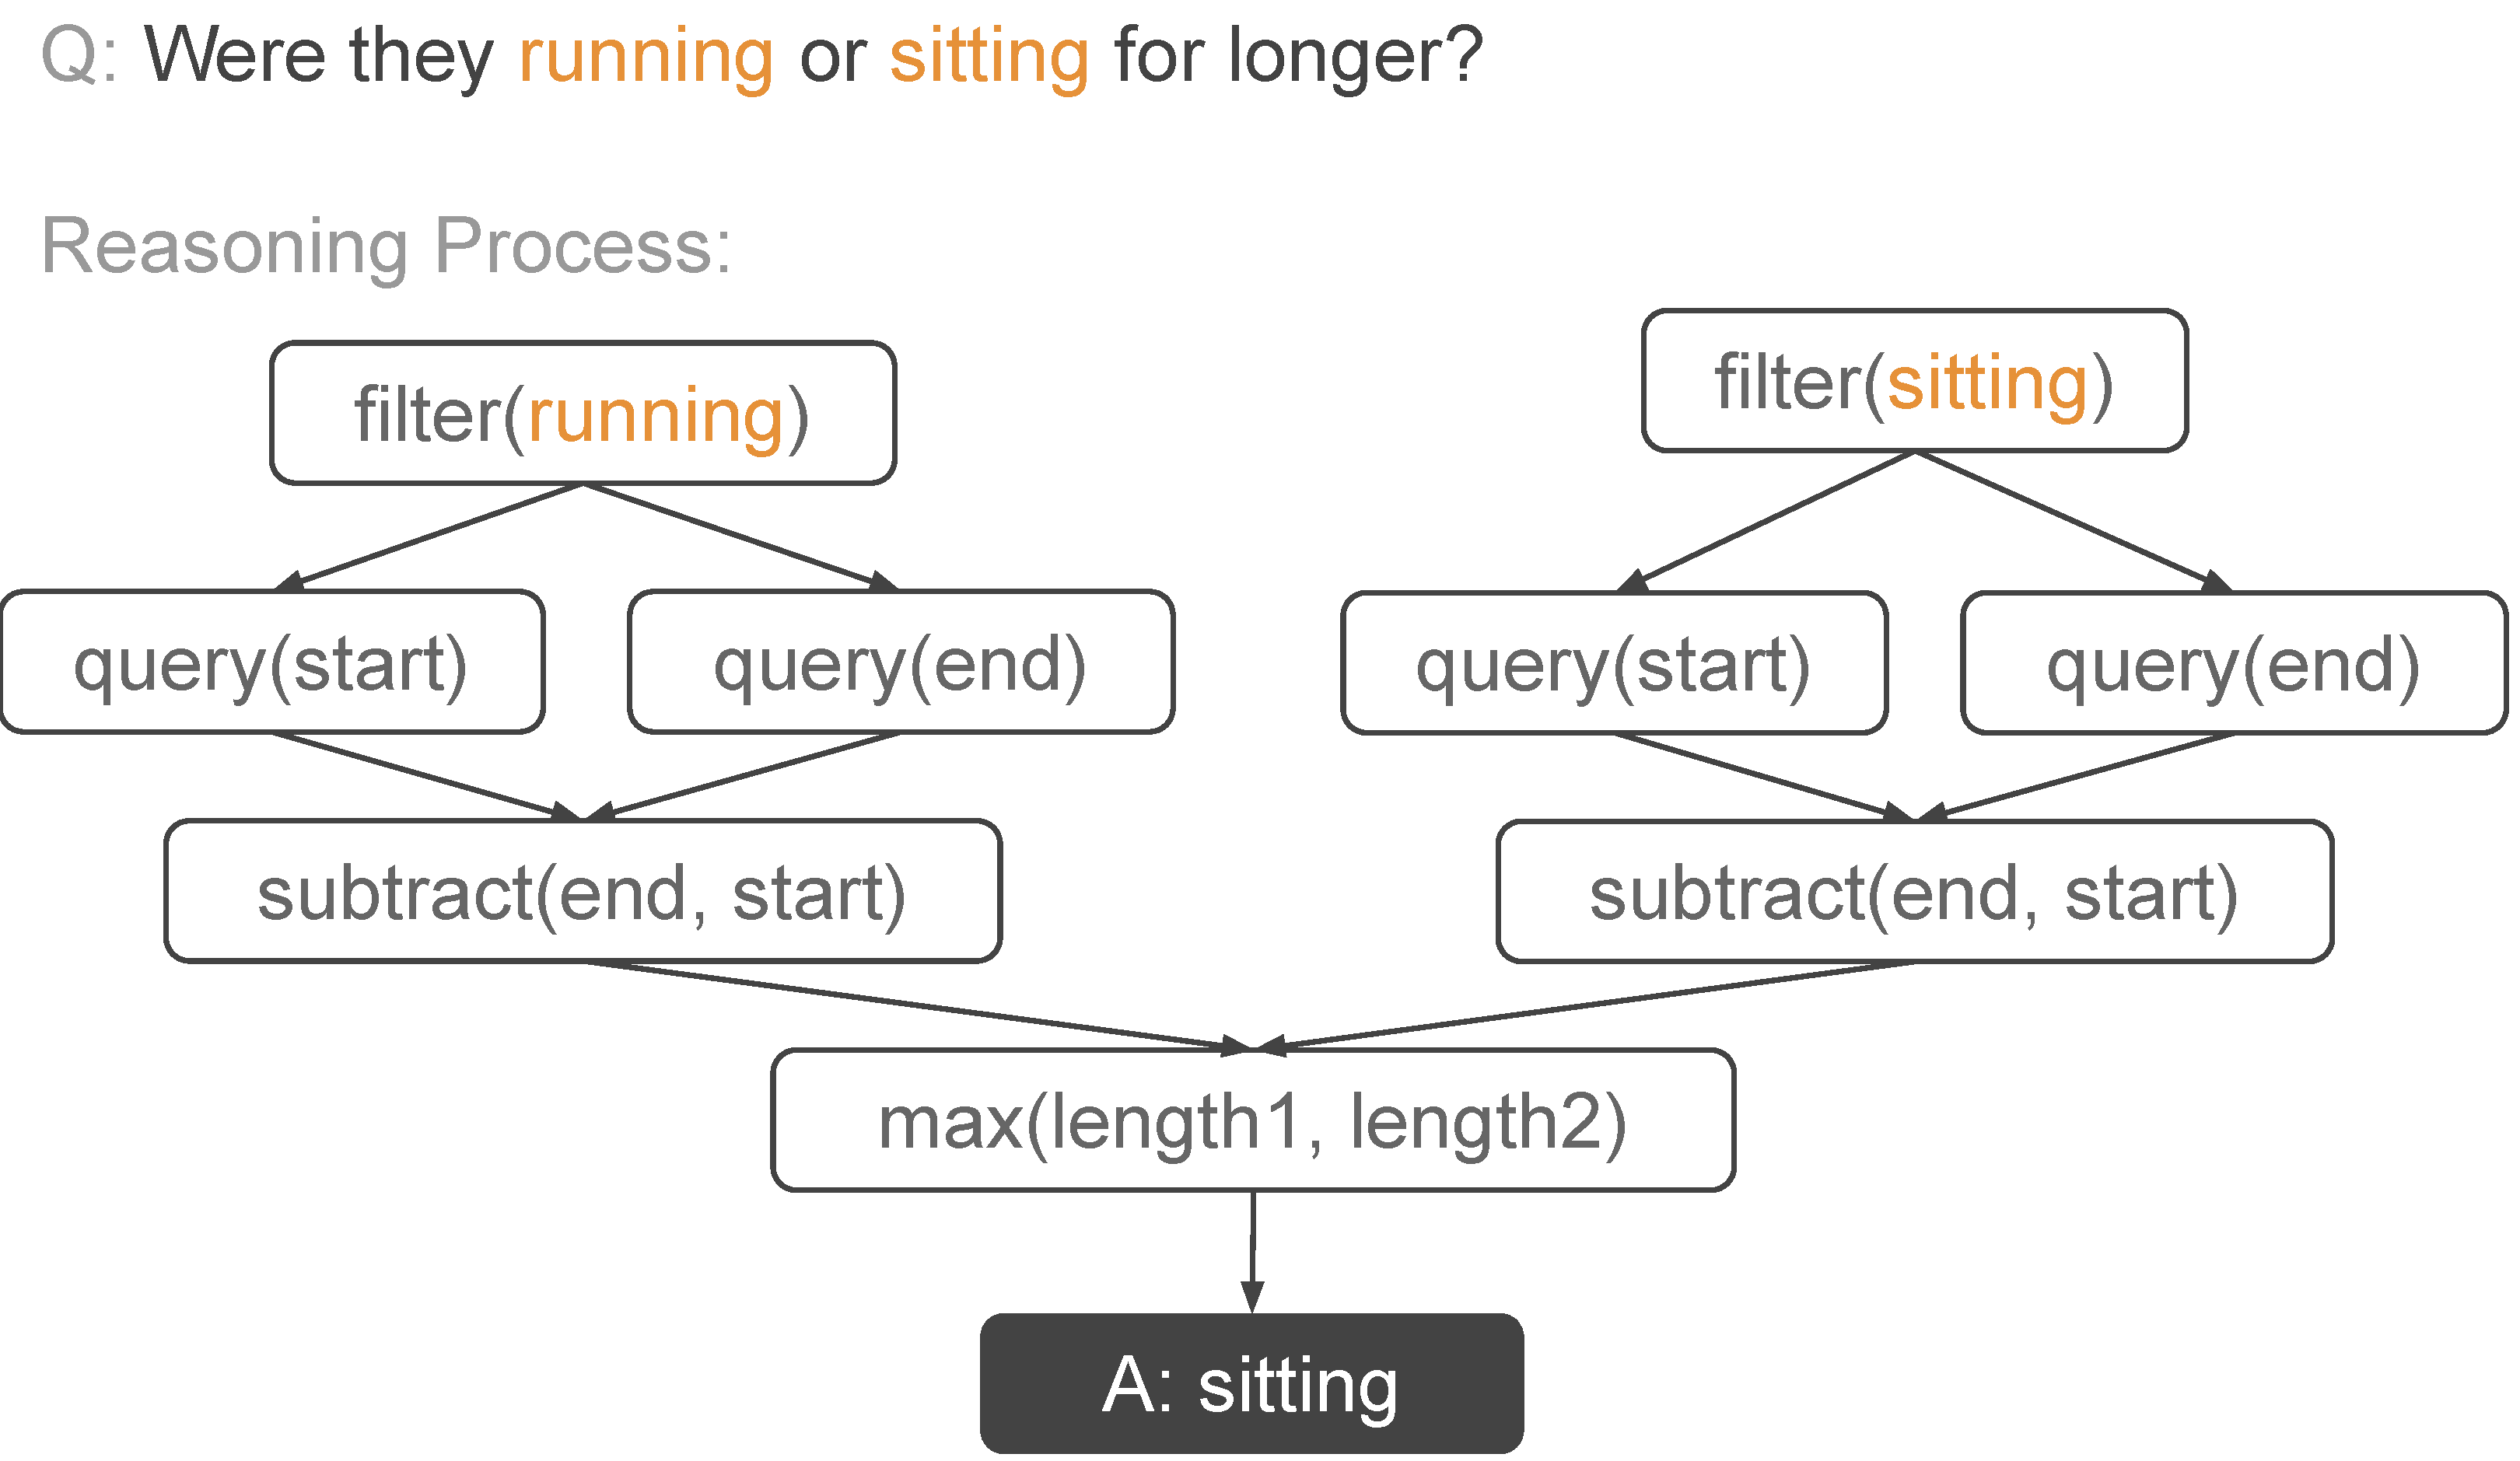
\includegraphics[width=0.95\linewidth]{figures/reasoning_tree.pdf}
    \caption{A single question requires a series of reasoning steps to answer. The question "Were they running or sitting for longer" first requires locating where the two actions occurred, processing their lengths and finally comparing the lengths.}
    \label{fig:tree}
\end{figure}

We introduce the Action Genome Question Answering (AGQA), a new benchmark for compositional spatio-temporal reasoning. AGQA is built upon a refined portion of Action Genome's spatio-temporal scene graphs~\cite{ji2020action}, which outlines the primitives 

\rak{TODO: working on this paragraph. The next couple of sentences are just random. ignore them}
To achieve these goals, we developed an automatic approach that converts Action Genome’s spatio-temporal scene graphs, containing objects, relationships, actors, and actions, into highly complex questions~\cite{ji2020action}. This process gives us tight control over the content of the questions to create a suite of metrics measuring individual spatio-temporal reasoning skills and compositional reasoning skills. We test AGQA on state-of-the art models to evaluate their strengths and weaknesses. 
By recursively generating questions with direct references, indirect references, and temporal localizations, our question generation pipeline creates a diverse set of questions that can be trained and tested all together or separated by type.


AGQA presents a balanced benchmark of $1.77$ million question answer pairs associated with $9.6K$ videos, along with an additional unbalanced set of $133M$ question answer pairs for future work to utilize. Each question is associated with a corresponding program, outlining the necessary visual reasoning steps require to answer the question (Figure~\ref{fig:tree}). These reasoning steps include identifying objects, understanding relationships and recognizing actions, which are each spatio-temporally grounded in the videos, using Action Genome~\cite{ji2020action}. AGQA contains multiple training and test splits, each testing for different forms of compositionality. These split tests how well models generalize to novel compositions they have not seen during training, or to videos longer than the ones in the training set or to questions with more compositional steps. Using AGQA, we evaluate modern visual reasoning systems~\cite{fan2019heterogeneous, le2020hierarchical, li2019beyond}, and find that the best model~\cite{} barely performs better than random chance of and it's improvements are largely due to exploiting language bias. We also find that while some models are able to generalize to videos of longer length, all of them are unable to generalize to questions with novel compositions unseen during training.


\begin{table*}[t]
\caption{A comparison of our AGQA with existing video question answering datasets. AGQA is orders of magnitude larger than all existing question answering datasets. It is also the first
large-scale real-world video question answering database providing both action, object, and relationship grounding.}
\label{tab:dataset_compare}
\resizebox{\linewidth}{!}{%
\begin{tabular}{@{\extracolsep{4pt}}l lrc ccccl ccc@{}}
 \multirow{2}{*}{Dataset} & \multicolumn{3}{c}{Video} & \multicolumn{4}{c}{Question answers} & \multicolumn{3}{c}{Grounding} \\ 
 \cline{2-4}\cline{5-8}\cline{9-11}
 & Avg. Length (s) & \# Videos (K) & Real-world & Not Dialogue Related & Open Answer & Compositional & \# QA Pairs & objects & relationships & actions \\ 
 \hline
MarioQA~\cite{mun2017marioqa} & 3-6 & 188 &  & \checkmark & \checkmark & & 188K \\
CLEVRER~\cite{yi2019clevrer} & 5 & 20 &  & \checkmark & \checkmark & \checkmark & 282K & \checkmark & \checkmark & \checkmark\\ \hline
Pororo-QA~\cite{kim2017deepstory} & 1.4 & 16.1 & \checkmark &  &  & & 9K \\
MovieQA~\cite{tapaswi2016movieqa}  & 202.7 & 6.77 & \checkmark &  &  & & 6.4K \\
SocialIQ~\cite{zadeh2019social} & 99 & 1.25 & \checkmark &  &  & & 7.5K \\
TVQA~\cite{lei2018tvqa} & 76.2 & 21.8 & \checkmark &  &  & \checkmark & 152.5K \\
MovieFIB\cite{maharaj2017dataset} & 4.9 & 118.5 & \checkmark & \checkmark & \checkmark & & 349K \\
TGIF-QA~\cite{jang2017tgif} & 3.1 & 71.7 & \checkmark & \checkmark & \checkmark & & 165.2K \\
MSVD-QA~\cite{xu2017video} & $<$10 & 1.97 & \checkmark & \checkmark & \checkmark & & 50.5K \\
Video-QA~\cite{zeng2016leveraging} & 45 & 18.1 & \checkmark & \checkmark & \checkmark & & 175K \\
MSRVTT-QA~\cite{xu2017video} & 10-30 & 10 & \checkmark & \checkmark & \checkmark & & 243K \\
ActivityNet-QA~\cite{yu2019activitynet} & 180 & 5.8 & \checkmark & \checkmark & \checkmark & & 58K \\
\hline
\textbf{AGQA} & 30 & 9.6 & \checkmark & \checkmark & \checkmark & \checkmark &  \textbf{1.7M} & \checkmark & \checkmark & \checkmark\\
\end{tabular}}
\end{table*}
